\chapter{Context}
\label{spec:ch:context}

This bachelor thesis is done by Simon Barras and supervised by Frederic Bapst and Jean Hennebert.
The customer Paolo Calafiura is a physicist and computer scientist at the \acrfull{lbl}.
To do this project, Simon Barras is moving to Berkeley, California, for ten weeks.
The goal is to improve the performance of the project Celeritas, which is a particle physics simulation software accelerated by \acrshort{gpu}s.




\section{Celeritas}
\label{spec:ch:context:celeritas}

The project Celeritas~\cite{Celeritas-Project} is a particle physics simulation software based on top of the Geant4~\cite{Geant4} project.
Geant4 is a toolkit for the simulation of the passage of particles through matter.
It is used by many simulation software in the field of particle physics.
The fact is that Geant4 is not accelerated by \acrshort{gpu}s and the aim of Celeritas is to optimize the performance of Geant4 by using \acrshort{gpu}s, specialy for the collision of photon.



\subsection{Physics Simulation}
\label{spec:ch:context:celeritas:physics-simulation}

This project simulate the path of the particule in the detector for an experiment made by the \acrfull{cern} with the \acrfull{lhc}.
The aim is to verrify that the measured data are correct but it also usefull to etalon the detector.
In fact, the simulation also help to compute the result error when due to a lack of precision.

To simulate the path of the particule, the software use the Monte Carlo Integration~\cite{Monte-Carlo-integration} and the Runge-Kutta method~\cite{Runge-Kutta-methods}.


\subsection{Lawrence Berkeley National Laboratory}
\label{spec:ch:context:celeritas:lbl}

The \acrfull{lbl} is a national laboratory in Berkeley, California.
It is managed and operated by the University of California for the \acrfull{doe}.
Since the lab take part of the \acrshort{doe}, it is a multidisciplinary research center that all the research are public and open source.
The lab is situated in the hills of Berkeley and it is composed of many buildings and has a beautifull view on the San-Fransisco bay \ref{spec:fig:context:lbl:lab-view}.

\begin{figure}[ht]
    \centering
    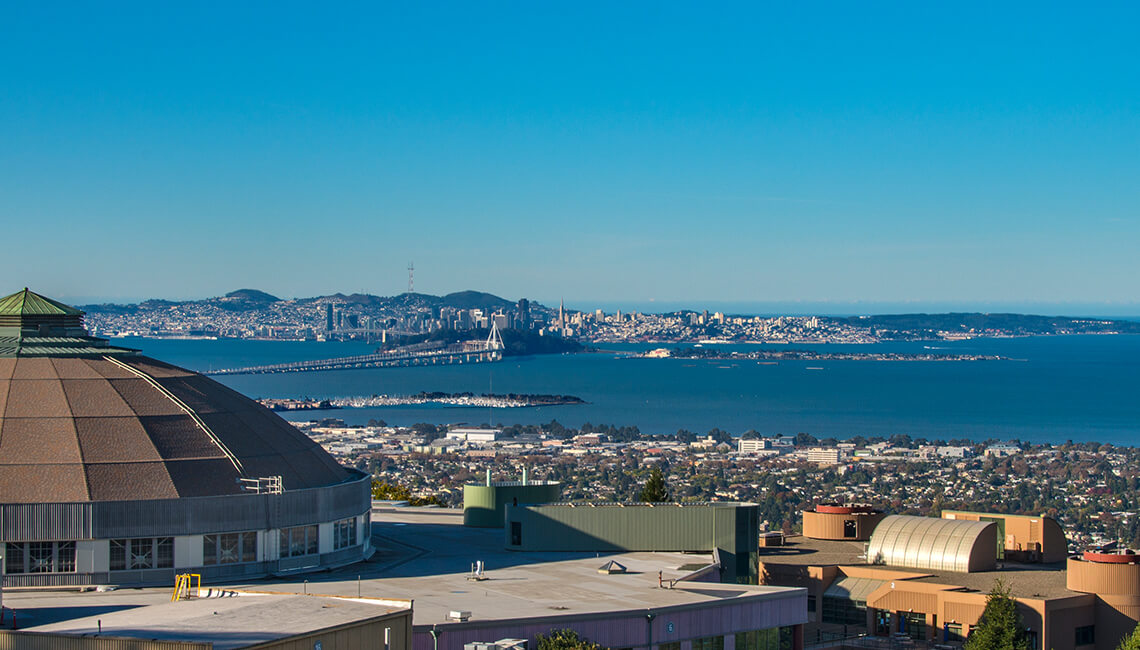
\includegraphics[width=0.8\textwidth]{05-resources/img/spec/lab-view.jpg}
    \caption{Lawrence Berkeley National Laboratory}
    \label{spec:fig:context:lbl:lab-view}
\end{figure}


The Physics and X-Ray Science Group, where the project is done, is situated in the building 50f.


\subsection{The Need}
\label{spec:ch:context:celeritas:need}

Celeritas already accelerate Geant4 by using \acrshort{gpu}s.
However, the team want to improve the performance to be able to reduce the time of simulation.
Before the bachelor thesis, the path of each particules is computed by a \acrshort{gpu} thread.
When the code is profiled, the distribution of the time is mainly occuped by two part of the code.
The first one is a Geant4 computation that cannot be accelerated by Celeritas.
The second one is the computation of the path using the Runge-Kutta method~\cite{Runge-Kutta-methods}.

